\subsection{Badania przy zmianie dwóch parametrów jednocześnie}

\begin{figure}[H]
	\centering
	\hspace*{-0.8in}
	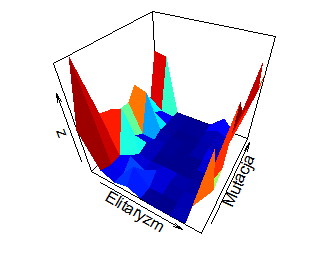
\includegraphics[scale = 1]{el_mut}
	\caption{Wykres dla własnej funkcji mutacji i selekcji elitarnej}  
	\label{rys:el_mut} 
\end{figure}

Na wykresie widać, że skrajne wartości parametrów powodują gorsze wyniki. Należy więc wybierać uśrednione wartości.